\documentclass[UTF8, a4paper, 11pt]{article}
\usepackage{amssymb}
\usepackage{fontspec}
\usepackage{float}
\usepackage{amsmath}
\newtheorem{myDef}{Definition}
\usepackage{graphicx}
\usepackage{geometry}
\usepackage{listings}
\usepackage{xcolor}
\usepackage{caption,subcaption}
\geometry{scale=0.8}
\linespread{1.5}
\usepackage{hyperref}
\usepackage{color}
\usepackage{fontspec}
\usepackage{enumitem}
\usepackage[linesnumbered,boxed]{algorithm2e}    
\usepackage{xeCJK}
\usepackage{indentfirst} 
\graphicspath{{Pic/}} 	% 在于.tex同级的目录下创建名为pic的文件夹,存放图片


\setlength{\parindent}{2em}


\lstset{
    language={C},
    frame=shadowbox,
    breaklines=true,
    numbers=left,
    backgroundcolor=\color[RGB]{245,245,244},
    rulesepcolor=\color{red!20!green!20!blue!20},
    numberstyle={\color[RGB]{0,192,192}\tiny},
    basicstyle=\footnotesize \fontspec{Source Code Pro}
}
\setenumerate[1]{itemsep=0pt,partopsep=0pt,parsep=\parskip,topsep=0pt}
\setitemize[1]{itemsep=0pt,partopsep=0pt,parsep=\parskip,topsep=0pt}
\setdescription{itemsep=0pt,partopsep=0pt,parsep=\parskip,topsep=0pt}


\title{	
\normalfont \normalsize
\textsc{School of Data and Computer Science, Sun Yat-sen University} \\ [25pt] %textsc small capital letters
\rule{\textwidth}{0.5pt} \\[0.4cm] % Thin top horizontal rule
\huge Reproduction of Generative Adversarial Self-Imitation Learning\\ % The assignment title
\rule{\textwidth}{2pt} \\[0.5cm] % Thick bottom horizontal rule
\author{18308045 Zhengyang Gu}
\date{\normalsize\today}
}

\begin{document}
\maketitle
\tableofcontents
\newpage

\section{Theories}
\subsection{Policy Gradient}
\subsubsection{On-policy}
The purpose of policy gradient is to maximize the expected reward as follows:
$$\overline R_\theta=\sum_\tau R(\tau)p_\theta(\tau)=E_{\tau\sim p_\theta}[R(\tau)]$$
where $R(\tau)$ is the final reward of trajectory $\tau$ and $p_\theta$ is the probability of trajectory $\tau$.Therefore, we need to calculate its gradient to do
gradient ascent. The gradient of it can be calculated by:
$$\begin{aligned}
\nabla\overline R_\theta=&\sum_\tau R(\tau)\nabla p_\theta(\tau)\\
=&\sum_\tau R(\tau)p_\theta(\tau)\frac{\nabla p_\theta(\tau)}{p_\theta(\tau)}\\
=&\sum_\tau R(\tau)p_\theta(\tau)\nabla\log(p_\theta(\tau))\\
=&\mathbb{E}_{\tau\sim p_\theta} R(\tau)\nabla\log(p_\theta(\tau))
\end{aligned}$$
We can estimate the expectation using sampling, so we have:
$$\begin{aligned}
\nabla\overline R_\theta\approx&\frac1 N\sum_{n=1}^N R(\tau^n)\nabla\log(p_\theta(\tau^n))\\
=&\frac1 N\sum_{n=1}^N\sum_{t=1}^{T_n}R(\tau^n)\nabla\log(p_\theta(a_t^n|s_t^n))
\end{aligned}$$
where $N$ is the total number of samples, and $\tau^n$ is the $n$th sampled trajectory. Since the $R(\tau^n)$ is always positive, a biased sampling may cause
unexpected ascent of some bad trajectories whose rewards are lower than average reward. Therefore, we can add a baseline to it to penalize those bad trajectories,
as follows:
$$\nabla\overline R_\theta\approx\frac1 N\sum_{n=1}^N\sum_{t=1}^{T_n}(R(\tau^n)-b)\nabla\log(p_\theta(a_t^n|s_t^n))$$
where $b$ can be easily assigned $\frac1 N\sum_{n=1}^N R(\tau^n)$. Additionally, we can separately evaluate each action given a state in a trajectory, so we have:
$$\begin{aligned}
\nabla\overline R_\theta\approx&\frac1 N\sum_{n=1}^N\sum_{t=1}^{T_n}A^\theta(s_t,a_t)\nabla\log(p_\theta(a_t^n|s_t^n))
\end{aligned}$$
where $A^\theta(s_t,a_t)$ is the advantage function to estimate the $\sum_{t'=t}^{T_n}\gamma^{t'-t}r_{t'}^n-b$.
\subsubsection{Off-policy}
Using on-policy policy gradient, we have to sample trajectories every time we update the policy to calculate the expectation, which is not data efficient. However,
we can exploit off-policy policy gradient to improve the data efficiency as follows:
$$\begin{aligned}
\mathbb{E}_{x\sim p}[f(x)]=&\sum_x p(x)f(x)\\
=&\sum_x q(x)\frac{p(x)}{q(x)}f(x)\\
=&\mathbb{E}_{x\sim q}[\frac{p(x)}{q(x)}f(x)]
\end{aligned}$$
The expectation of off-policy policy gradient, thouth, is the same as on-policy gradient, the variance is very different. The variance of on-policy gradient is:
$$Var_{x\sim p}[f(x)]=\mathbb{E}_{x~p}[f(x)^2]-(\mathbb{E}_{x\sim q}[f(x)])^2$$
, while the variance of off-policy gradeint is:
$$\begin{aligned}
Var_{x\sim q}[\frac{p(x)}{q(x)}f(x)]=&\mathbb{E}_{x\sim q}[(\frac{p(x)}{q(x)}f(x))^2]-(\mathbb{E}_{x\sim q}[\frac{p(x)}{q(x)}f(x)])^2\\
=&\mathbb{E}_{x\sim p}[\frac{p(x)}{q(x)}(f(x))^2]-(\mathbb{E}_{x\sim p}[f(x)])^2
\end{aligned}$$
, which means if the $p(x)$ and $q(x)$ differ a lot, the variance of them can differ a lot. To solve the problem, there are several algorithm such as PPO, TRPO and
PPO2 etc.
\subsubsection{PPO2}
Here I will emphasize the PPO2 which has a slightly simpler form which makes it much easier to calculate loss than other than that of other two algorithms. The loss
of it has the form as follows:
$$\begin{aligned}
J_{PPO2}^{\theta^k}\approx\sum_{(s_t,a_t)}\min(&\frac{p_\theta(a_t|s_t)}{p_{\theta^k}(a_t|s_t)}A^{\theta^k}(s_t,a_t),\\
&clip(\frac{p_\theta(a_t|s_t)}{p_{\theta^k}(a_t|s_t)}A^{\theta^k}(s_t,a_t)))
\end{aligned}$$
When doing gradient ascent, if $A^{\theta^k}>0$, we have to increase the policy $p_{\theta}(a_t|s_t)$; if $A^{\theta^k}<0$, we have to decrease the pocliy
$p_{\theta}(a_t|s_t)$. However, when changing the policy $p_{\theta}(a_t|s_t)$, it won't differ a lot from the original policy $p_{\theta^k}(a_t|s_t)$ since the
limitation of bounds $(1-\epsilon)p_{\theta^k}(a_t|s_t)$ and $(1+\epsilon)p_{\theta^k}(a_t|s_t)$.
\begin{figure}[H]
    \centering
    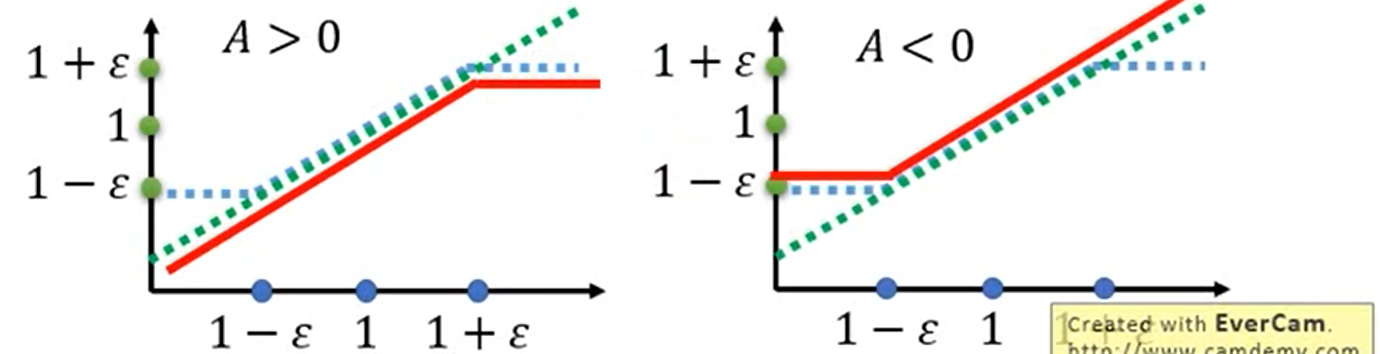
\includegraphics[width = \textwidth]{PPO2.png}
\end{figure}
\subsection{GAN}
The objective of GAN is to acquire an implicit generative model which is a generative probability distribution that is similar to the actual probability distribution.
The idea behind it is exploiting a confrontation between a discriminator and a generator, where the discriminator's job is to identify whether a set of samples are
from actual or generative probability distribution, while the generator's job is to generate a set of vivid samples to fool the discriminator. GAN's loss function is
actually a binary cross entropy loss for the discriminator, which has the form as follows:
$$\begin{aligned}
    L=&\frac1{2N}\sum_{i=1}^{2N}-(y_i\log(D(x_i))+(1-y_i)\log(1-D(x_i)))\\
    =&\frac1{2N}\sum_{i=1}^{2N}
    \begin{cases}
        -\log(D(x_i)),&y_i=1\\
        -\log(1-D(G(z_i))),&y_i=0
    \end{cases}\\
\end{aligned}$$
where $2N$ is the number of samples, $(x_i,y_1)$ is the $(feature, classification)$ pair, $D$ is the the possibility predicted by discriminator that the $x_i$ is
sampled from actual probability distribution, and $G$ is the generator network which is a part of implicit generative model. Assuming that half of the samples are
actual while the other half of the samples are generated, we have:
$$\begin{aligned}
    L=&\frac1{2N}\sum_{j=1}^{N}-\log(D(x_j))+\frac1{2N}\sum_{k=1}^{N}-\log(1-D(G(z_k)))\\
\end{aligned}$$
Then we define that $x~p$ is the actual possibility distribution while $z~q$ is the generative possibility distribution. Therefore, about $Np(x)$ $x_j$s are equal to
$x$ and about $Nq(z)$ $z_k$s are equal to $z$, so the $L$ can be written as the following form:
$$\begin{aligned}
    L\approx&\frac1{2N}\sum_x Np(x)(-\log(D(x)))+\frac1{2N}\sum_z Nq(z)(-\log(1-D(G(z))))\\
    =&\frac1 2\mathbb{E}_{x\sim p}[-\log(D(x))]+\frac1 2\mathbb{E}_{z\sim q}[-\log(1-D(G(z)))]
\end{aligned}$$
The higher the binary cross entropy is, the better the classification between actual samples and generated samples are. Therefore, the discriminator wants to
maxizmize the loss, while the generator wants to minimize the loss.
\subsection{GASIL}
GASIL is actually a kind of GAN. The only difference between it and other GANs is that the actual samples here are historical good trajectories and the generative
probability distribution here is trained policy. And it also exploit entropy regularization to prevent the loss function dropping into locally optimal point.
Therefore, the loss function of it has the following form:
$$L_{GASIL}(\theta,\phi)=\mathbb{E}_{\pi_\theta}[\log(D_{\phi}(s,a))]+E_{\pi_E}[\log(1-D_\phi(s,a))]-\lambda H(\pi_\theta)$$
The training algorithm can be written as follows:
\begin{figure}[H]
    \centering
    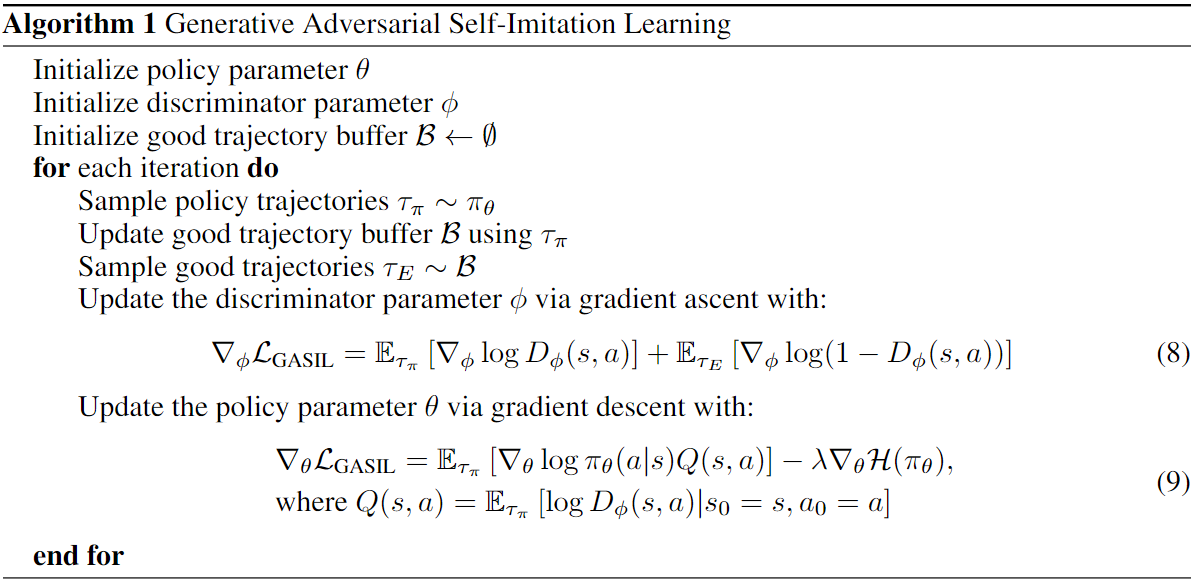
\includegraphics[width = \textwidth]{algorithm.png}
\end{figure}
where the good trajectories here are defined as historical top-K trajectories, and the gradient with respect to $\theta$ is actually to calculate the expectation's
gradient, which is discussed in the policy gradient section. Since the similarity between the policy's training and policy gradient, the $\log(D_\phi(s,a))$ here can be
regarded as a reward of an action $a$ given a state $s$. Therefore, GASIL can be easily combined with some policy gradient algorithms. So we can update the policy
parameter $\theta$ via gradient ascent with:
$$\nabla_\theta J_{PG}-\alpha\nabla_\theta L_{GASIL}=\mathbb{E}_{\pi_\theta}[\nabla_\theta\log(\pi_\theta(a|s)\hat A_t^\alpha)]$$
where $\hat A_t^\alpha$ is an advantage estimation using a modified reward function $r^\alpha(s,a)=r(s,a)-\alpha\log(D_\phi(s,a))$.
\section{Implementation}
\subsection{PPO2}
The pseudo algorithm is shown as below:
\begin{figure}[H]
    \centering
    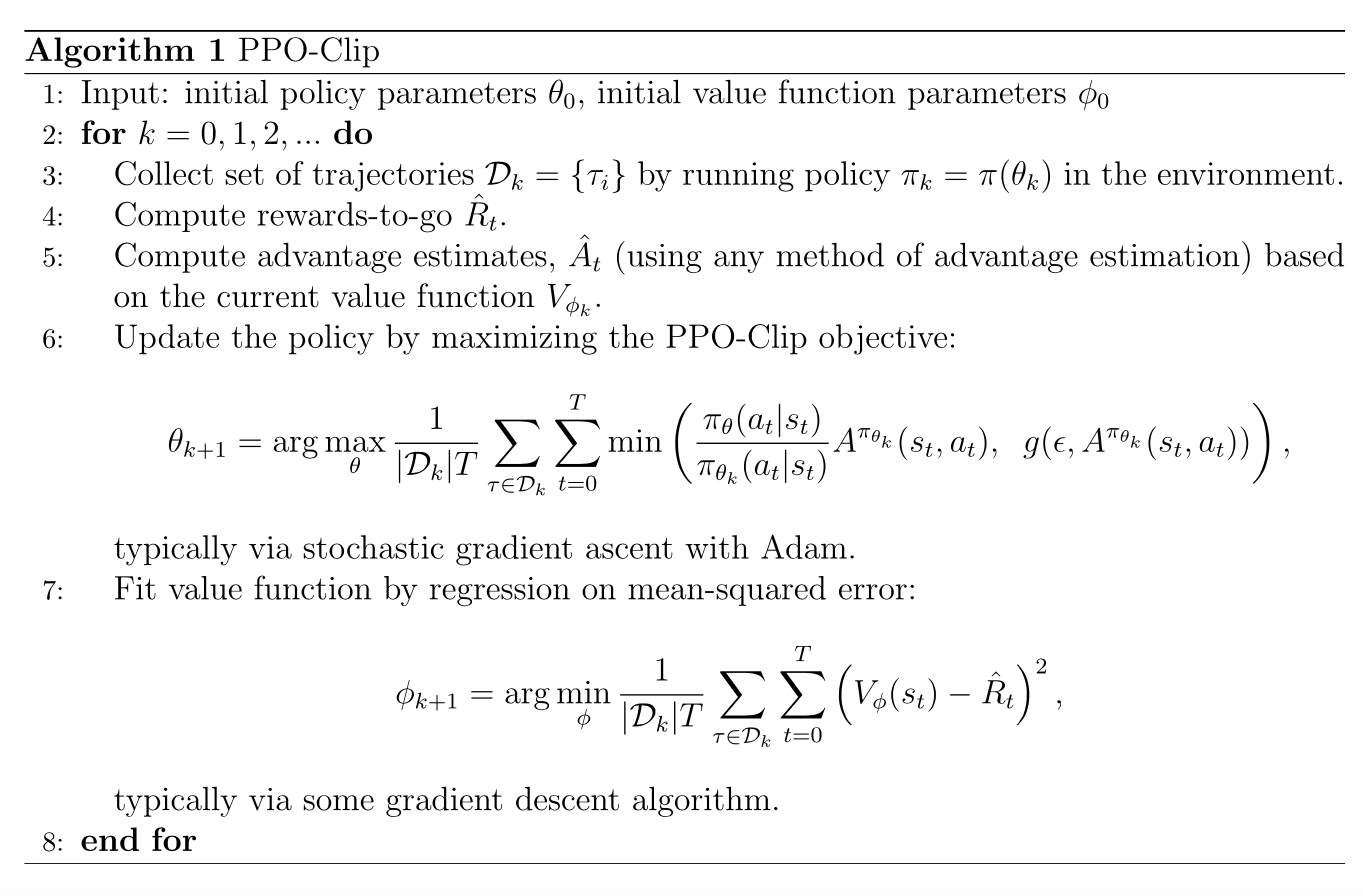
\includegraphics[width = \textwidth]{PPO-Clip.png}
\end{figure}
Inspired by \href{https://medium.com/analytics-vidhya/coding-ppo-from-scratch-with-pytorch-part-1-4-613dfc1b14c8}{Coding PPO From Scratch With PyTorch}, I translated
each step of the algorithm into codes.

The first step is to create the actor and critic network
\begin{figure}[H]
    \centering
    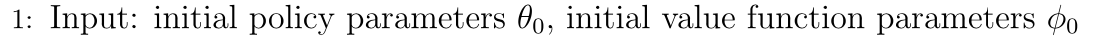
\includegraphics[width = \textwidth]{step1.png}
\end{figure}
, which can be simply translated into:
\begin{lstlisting}
# ALG STEP 1
# Initialize actor and critic networks
self.actor = Policy(self.obs_dim, self.act_dim).to(self.device)
self.critic = Value(self.obs_dim).to(self.device)
\end{lstlisting}
, where Policy and Value are networks defined in mlp\_policy.py and mlp\_critic.py repectively.

The second step is to implement a loop structure:
\begin{figure}[H]
    \centering
    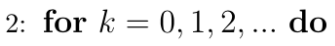
\includegraphics[width = 0.4\textwidth]{step2.png}
\end{figure}
We need to define some variables that can be increased to implement the loop structure.
\begin{lstlisting}
pbar = tqdm(total=self.total_timesteps)
while self.t_so_far < self.total_timesteps: # ALG STEP 2
    ...
    # Calculate how many timesteps we collected this batch
    delta_t = np.sum(self.batch_lens)
    self.t_so_far += delta_t
    pbar.update(delta_t)

    # Increment the number of iterations
    self.i_so_far += 1
\end{lstlisting}
The third and forth step are to collect trajectories and calculate their rewards-to-go:
\begin{figure}[H]
    \centering
    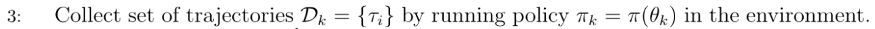
\includegraphics[width = \textwidth]{step3.png}
    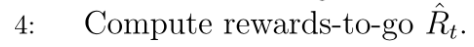
\includegraphics[width = 0.4\textwidth]{step4.png}
\end{figure}
I implemented them in the function called rollout. Since there are no dependencies among all the samples, we can do sampling in parallel:
\begin{lstlisting}
# Number of timestpes run so far this batch
t = 0
for pid in range(1, self.max_num_threads):
    workers.append(threading.Thread(target=self.env_thread, args=(pid, thread_batch_size)))
    t += thread_batch_size
    workers[-1].start()
self.env_thread(0, self.timesteps_per_batch - t)
for worker in workers:
    worker.join()
\end{lstlisting}
After all threads' sampling, we have to gather all the samples sampled by these threads. And the gathering can also be done in parallel:
\begin{lstlisting}
List_list = [self.batch_obs, self.batch_acts, self.batch_log_probs, self.batch_rews, self.batch_rtgs, self.batch_lens]
pid = 0
while pid < 6:
    workers = []
    first_pid = pid
    for pid in range(first_pid + 1, min(6, first_pid + self.max_num_threads)):
        workers.append(threading.Thread(target=self.extend_thread, args=(List_list[pid],)))
        workers[-1].start()
    pid += 1
    self.extend_thread(List_list[first_pid])
    for worker in workers:
        worker.join()
\end{lstlisting}
, where each thread gathers one of the six kinds of results in List\_list.

Rewards-to-go is actually discounted sum of rewards, which is done by the function compute\_rtgs:
\begin{lstlisting}
def compute_rtgs(self, ep_rews):
    # The rewards-to-go (rtg) per episode to return.
    # The shape will be (num timesteps per episode)
    ep_rtgs = []
    discounted_reward = 0 # The discounted reward so far
    for rew in reversed(ep_rews):
        discounted_reward = rew + discounted_reward * self.gamma
        ep_rtgs.append(discounted_reward)
    return list(reversed(ep_rtgs))
\end{lstlisting}
The fifth step is to compute the advantage estimates:
\begin{figure}[H]
    \centering
    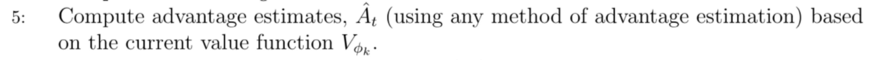
\includegraphics[width = \textwidth]{step5.png}
\end{figure}
, which can be simply translated into:
\begin{lstlisting}
# Calculate V_{phi, k}
V, _ = self.evaluate()

# ALG STEP 5
# Calculate advantage
A_k = self.batch_rtgs - V.detach()

# Normalize advantages
A_k = (A_k - A_k.mean()) / (A_k.std() + 1e-10)
\end{lstlisting}
, where V is the baseline estimated by critic network mentioned above.

The final two steps respectively update the two networks:
\begin{figure}[H]
    \centering
    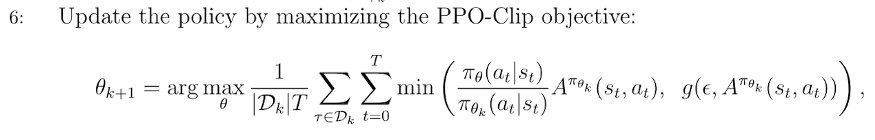
\includegraphics[width = \textwidth]{step6.png}
    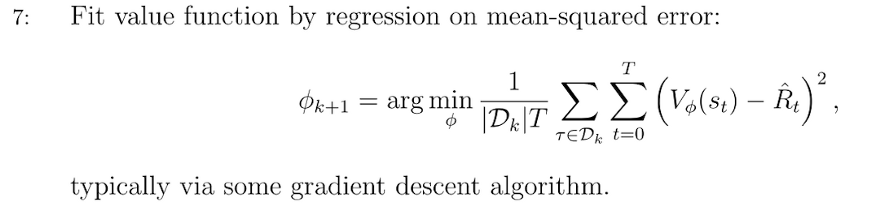
\includegraphics[width = \textwidth]{step7.png}
\end{figure}
, which can be simply written as:
\begin{lstlisting}
# Calculate surrogate losses
surr1 = ratios * A_k
surr2 = torch.clamp(ratios, 1 - self.clip, 1 + self.clip) * A_k
# Calculate actor loss
actor_loss = -((torch.min(surr1, surr2) - self.Lambda * ratios * curr_log_probs).mean())

# Calculate gradients and perform backward propagation for actor network
self.actor_optim.zero_grad()
actor_loss.backward(retain_graph=True)
self.actor_optim.step()

# Calculate critic loss
critic_loss = self.critic_criterion(V, self.batch_rtgs)

# Calculate gradients and perform backward propagation for critic network
self.critic_optim.zero_grad()
critic_loss.backward()
self.critic_optim.step()
\end{lstlisting}
, where the (- self.Lambda * rations * curr\_log\_probs).mean() is actually the entropy regularization$-\lambda H(\pi_\theta)$.
\subsection{GASIL}
The pseudo algorithm is shown as below:
\begin{figure}[H]
    \centering
    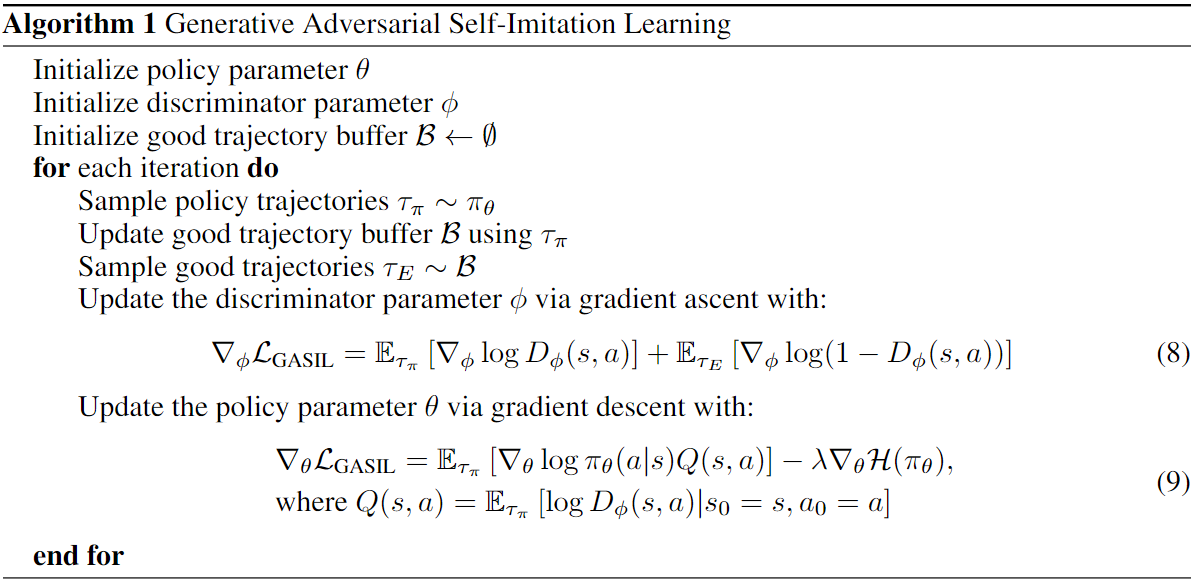
\includegraphics[width = \textwidth]{algorithm.png}
\end{figure}
GASIL can be devided into two parts. The first part is to update the discriminator. The second part is to update the policy, which is actually done by PPO. The
connection between these two parts is that the rewards of each action here is modified reward function $r^\alpha(s,a)=r(s,a)-\alpha\log(D_\phi(s,a))$. Therefore the
rewards-to-go should be computed using the modified rewards.

When it comes to the discriminator, we have to sample trajectories from current policy and historical good trajectories respectively. Sampling from current policy is
similar to that of PPO, while sampling from historical good trajectories requires us to maintain a buffer of these good trajectories. I use the priority queue to
implement the buffer, where the top of the heap has the lowest unmodified rewards-to-go.
\begin{lstlisting}
# Initialize good trajectory buffer B
self.B = PriorityQueue()
\end{lstlisting}
And the max size of the buffer is K, which is set as a hyperparameter:
\begin{lstlisting}
if 'K' in conf: # size of good trajectory buffer B
    self.K = conf['K']
else:
    self.K = 10
\end{lstlisting}
Each time we sample a new trajectory from current policy, we have to update the buffer:
\begin{lstlisting}
# Update good trajectory buffer B using \Tau_\pi
self.B.put(GoodTrajectory(ep_obs, ep_acts, np.mean(ep_rtgs_actual)))
if self.B.qsize() > self.K:
    self.B.get()
\end{lstlisting}
And since we just want those trajectories that are better than the current policy's average level, we also have to remove those trajectories that have lower
unmodified rewards-to-go than the average rewards-to-go from the buffer.
\begin{lstlisting}
# Update good trajectory buffer B using \Tau_\pi
worst = self.B.get()
batch_rtgs_mean = np.mean(batch_rtgs_actual)
while worst.R <= batch_rtgs_mean:
    worst = self.B.get()
self.B.put(worst)
\end{lstlisting}
Sampling from buffer can be simply written as:
\begin{lstlisting}
# Sample good trajectories \Tau_E ~ B
B = [self.B.get() for _ in range(self.B.qsize())]
print('\nB_len_max_min:\t', len(B), max([b.R for b in B]), min([b.R for b in B]))
batch_E = np.random.choice(B, size=len(self.batch_lens), replace=True)
for E in B:
    self.B.put(E)

# Reshape data as tensors in the shape specified before returning
self.batch_E_obs = list()
self.batch_E_acts = list()
for E in batch_E:
    self.batch_E_obs.append(E.obs)
    self.batch_E_acts.append(E.acts)
self.batch_E_obs = torch.cat(self.batch_E_obs).to(self.device)
self.batch_E_acts = torch.cat(self.batch_E_acts).to(self.device)
\end{lstlisting}
The loss for the discriminator is actually the cross entropy. Therefore the updating of discriminator can be written as:
\begin{lstlisting}
# Initialize discriminator criterion
self.D_criterion = nn.BCELoss()
\end{lstlisting}
\begin{lstlisting}
# Update the discriminator \phi via gradient ascent with:
for _ in range(self.n_updates_of_D_per_iteration):
    g_o = self.D(torch.cat([self.batch_obs, self.batch_acts], 1))
    e_o = self.D(torch.cat([self.batch_E_obs, self.batch_E_acts], 1))
    self.D_optim.zero_grad()
    discrim_loss = self.D_criterion(g_o, torch.ones((self.batch_obs.shape[0], 1), device=self.device)) + \
        self.D_criterion(e_o, torch.zeros((self.batch_E_obs.shape[0], 1), device=self.device))
    discrim_loss.backward()
    self.D_optim.step()
\end{lstlisting}
When it comes to the second part, we can make the GASIL class to inherit the PPO class, and encapsulate the updating of PPO as a method of the PPO class. Therefore,
the second part is just call the method:
\begin{lstlisting}
self.ppo_update()
\end{lstlisting}
The only difference between the GASIL's calling ppo\_update and PPO's calling ppo\_update is that GASIL uses the modifeid rewards-to-go:
\begin{lstlisting}
# Modified reward function
ep_rtgs = self.compute_rtgs(np.array(ep_rews) - self.alpha_func(self.i_so_far) * self.D(torch.cat([ep_obs, ep_acts], 1)).detach().squeeze(1).numpy())
self.batch_rtgs.extend(ep_rtgs)
\end{lstlisting}
And a very interesting point here is that the authors didn't tell us how to set the weight $\alpha$, so I make the $\alpha$ a function which takes the number of
iterations so far as inputs. Therefore the $\alpha$ can be a constant or a increasing number.
\section{Experiments}
Due to the limitation of time, I just tested the PPO and the GASIL on only one task:
\begin{lstlisting}
conf = {'env': 'BipedalWalker-v3', 'device': 'cuda', 'seed': 0}
\end{lstlisting}
And I choose a relatively good set of values of hyperparameters, which are set as default values in function \_init\_hyperparameters. Particulaly, I set the $\alpha$
as $e^{\min(i,1000)-1000}$. The benefit of it is that it devides the training process into 2 phases. At first $\alpha\approx0$, so the policy tends to obtain higher
rewards. Therefore the buffer won't be too biased towards some locally optimal solution. Then $\alpha$ gets larger gradually, so the policy tends to imitate those
trajectories in the buffer. Therefore the policy can learn from various good solutions in the buffer.
\begin{figure}[H]
    \centering
    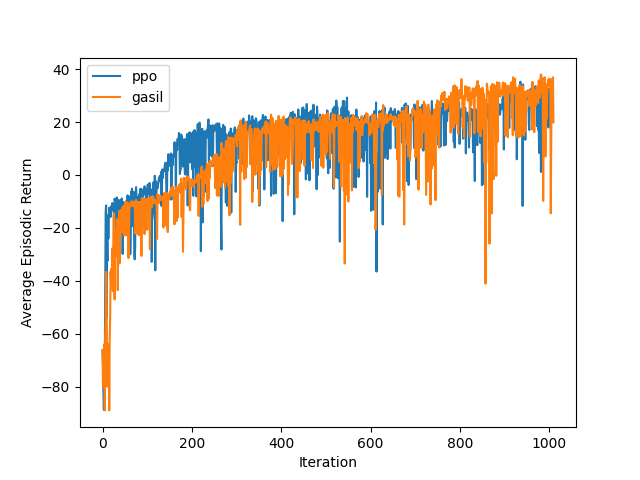
\includegraphics[width = \textwidth]{Figure_1.png}
\end{figure}
The result shows that PPO2 performs better at first though, GASIL's performance gradually exceeds that of PPO2. And there are two videos that directly show the models
trained by \href{run:./Vid/ppo.mp4}{PPO} and \href{run:./Vid/gasil.mp4}{GASIL}.
\section{Summary}
Since the limitation of the time, the comparison between PPO and GASIL is not as good as expected. The GASIL's advantages over PPO in my opinion is that its
hyperparameters is a superset of the PPO. And the imitation of perviously good trajectories makes it less likely fall into locally optimal solution. However there
seems not to be much locally optimal solution in this task, so the advantage of GASIL isn't shown much.

My future work may include trying various combination of values of hyperparameters, testing the algorithms on more tasks and introducing model based method into the
GASIL.
%\clearpage
%\bibliography{E:/Papers/LiuLab}
%\bibliographystyle{apalike}
\end{document}
%%% Local Variables:
%%% mode: latex
%%% TeX-master: t
%%% End:
